\section{Ausarbeitung des Alarmszenarios}

In dem nun folgenden Kapitel werden die Ergebnisse der Ausarbeitung vorgestellt. Zunächst werden wiederkehrende Begriffsdefinitionen geboten, um Kernelemente des Alarmszenarios zu spezifizieren und voneinander abzugrenzen. Anschließend wird der grundlegende Ablauf des MVPs erläutert.

\subsection{Begriffsabgrenzung}

Die nachfolgenden Begriffe stellen zentrale Elemente dar, welche im Kontext der Alarmsimulation zusammenwirken:

\begin{description}
    \item [\textbf{Übungsteilnehmer:}] 
     Person, welche die Alarmsimulation an einer angebundenen Industrie 4.0 Simulationsanlage durchläuft und Versuche unternimmt, die simulierte Störung in kürzester Zeit zu beheben. 

     \item [\textbf{Übungsleiter:}] 
    Person, welche die Administration der Alarmsimulation verantwortet und Szenarioart, als auch Zeitdauer von Eskalationsstufen individuell konfiguriert.

    \item [\textbf{Immersionsobjekt:}] 
   Objekt, welches nach Adressierung durch die Ablauflogik übermittelte Immersionseffekte durchführt. Dieses Objekt, beispielsweise ein Lautsprecher, kann etwa Brandgeräusche emittieren und sorgt für eine stärkere Immersion der Simulation auf den Übungsteilnehmer.

   \item [\textbf{Simulationstablett:}] 
   Zentrales Steuerungs- und Kommunikationselement für den Übungsteilnehmer, um die Entstörung durch Eingaben auf Tablet zu realisieren.

    \item [\textbf{Entstörungsvorgang:}] 
    Phase in der Ablauflogik, in der durch den Übungsteilnehmer versucht wird, die Störung durch das Lösen eines szenarionahen Rätels zu beheben. Der Entstörungsvorgang kann dabei erfolgreich, als auch unerfolgreich verlaufen.
   
   \item [\textbf{Eskalationsstufe:}] 
   Phase in der Simulation eines Szenarios, in welcher eine bestimmte Ausprägung von Immersionseffekten als auch Störungsbild gegeben ist. Eine Eskalationsstufe steht dabei in einer Rangfolge beziehungsweise Stufe zu anderen Eskalationsstufen, um eine Verstärkung des Immersionseffektes im Zeitverlauf der Simulation zu realisieren.
\end{description}

\subsection{Szenario}

Als \textit{MVP} Szenario wurde sich für die Simulation des Brandes einer Maschine im Kontext des \textit{Zentrums Industrie 4.0} entschieden. In den anschließenden Unterabschnitten wird beginnend der Ablauf des \textit{MVP} Szenarios skizziert und die einzelnen Eskalationsstufen dargelegt. Darauf folgend werden zusammengehörige Entstörungsvorgänge erläutert und ein Einblick in die Administration der Alarmszenarien geboten. Abschließend werden Begleitdokumente zur Unterstützung der Übungsteilnehmer und des Übungsleiters vorgestellt und ein Gesamtüberblick mithilfe eines aufgestellten Prozessmodells (siehe Kapitel \ref{chap:process model}) geboten.

\subsubsection{Ablauf}

Vor Start der Simulation des MVPs \textit{Maschinenbrand} ist durch den Übungsleiter sicherzustellen, dass die Anlage im \textit{Zentrum Industrie 4.0} aktiviert ist. Auf dem Tablet in der Administrationsoberfläche des Übungsleiters ist der Button \textit{Szenario starten} zu klicken, um das Szenario für den Übungsteilnehmer zu starten. In folgender Abbildung ist die Startoberfläche eines Übungsteilnehmers zu sehen:

\begin{figure}[h]
    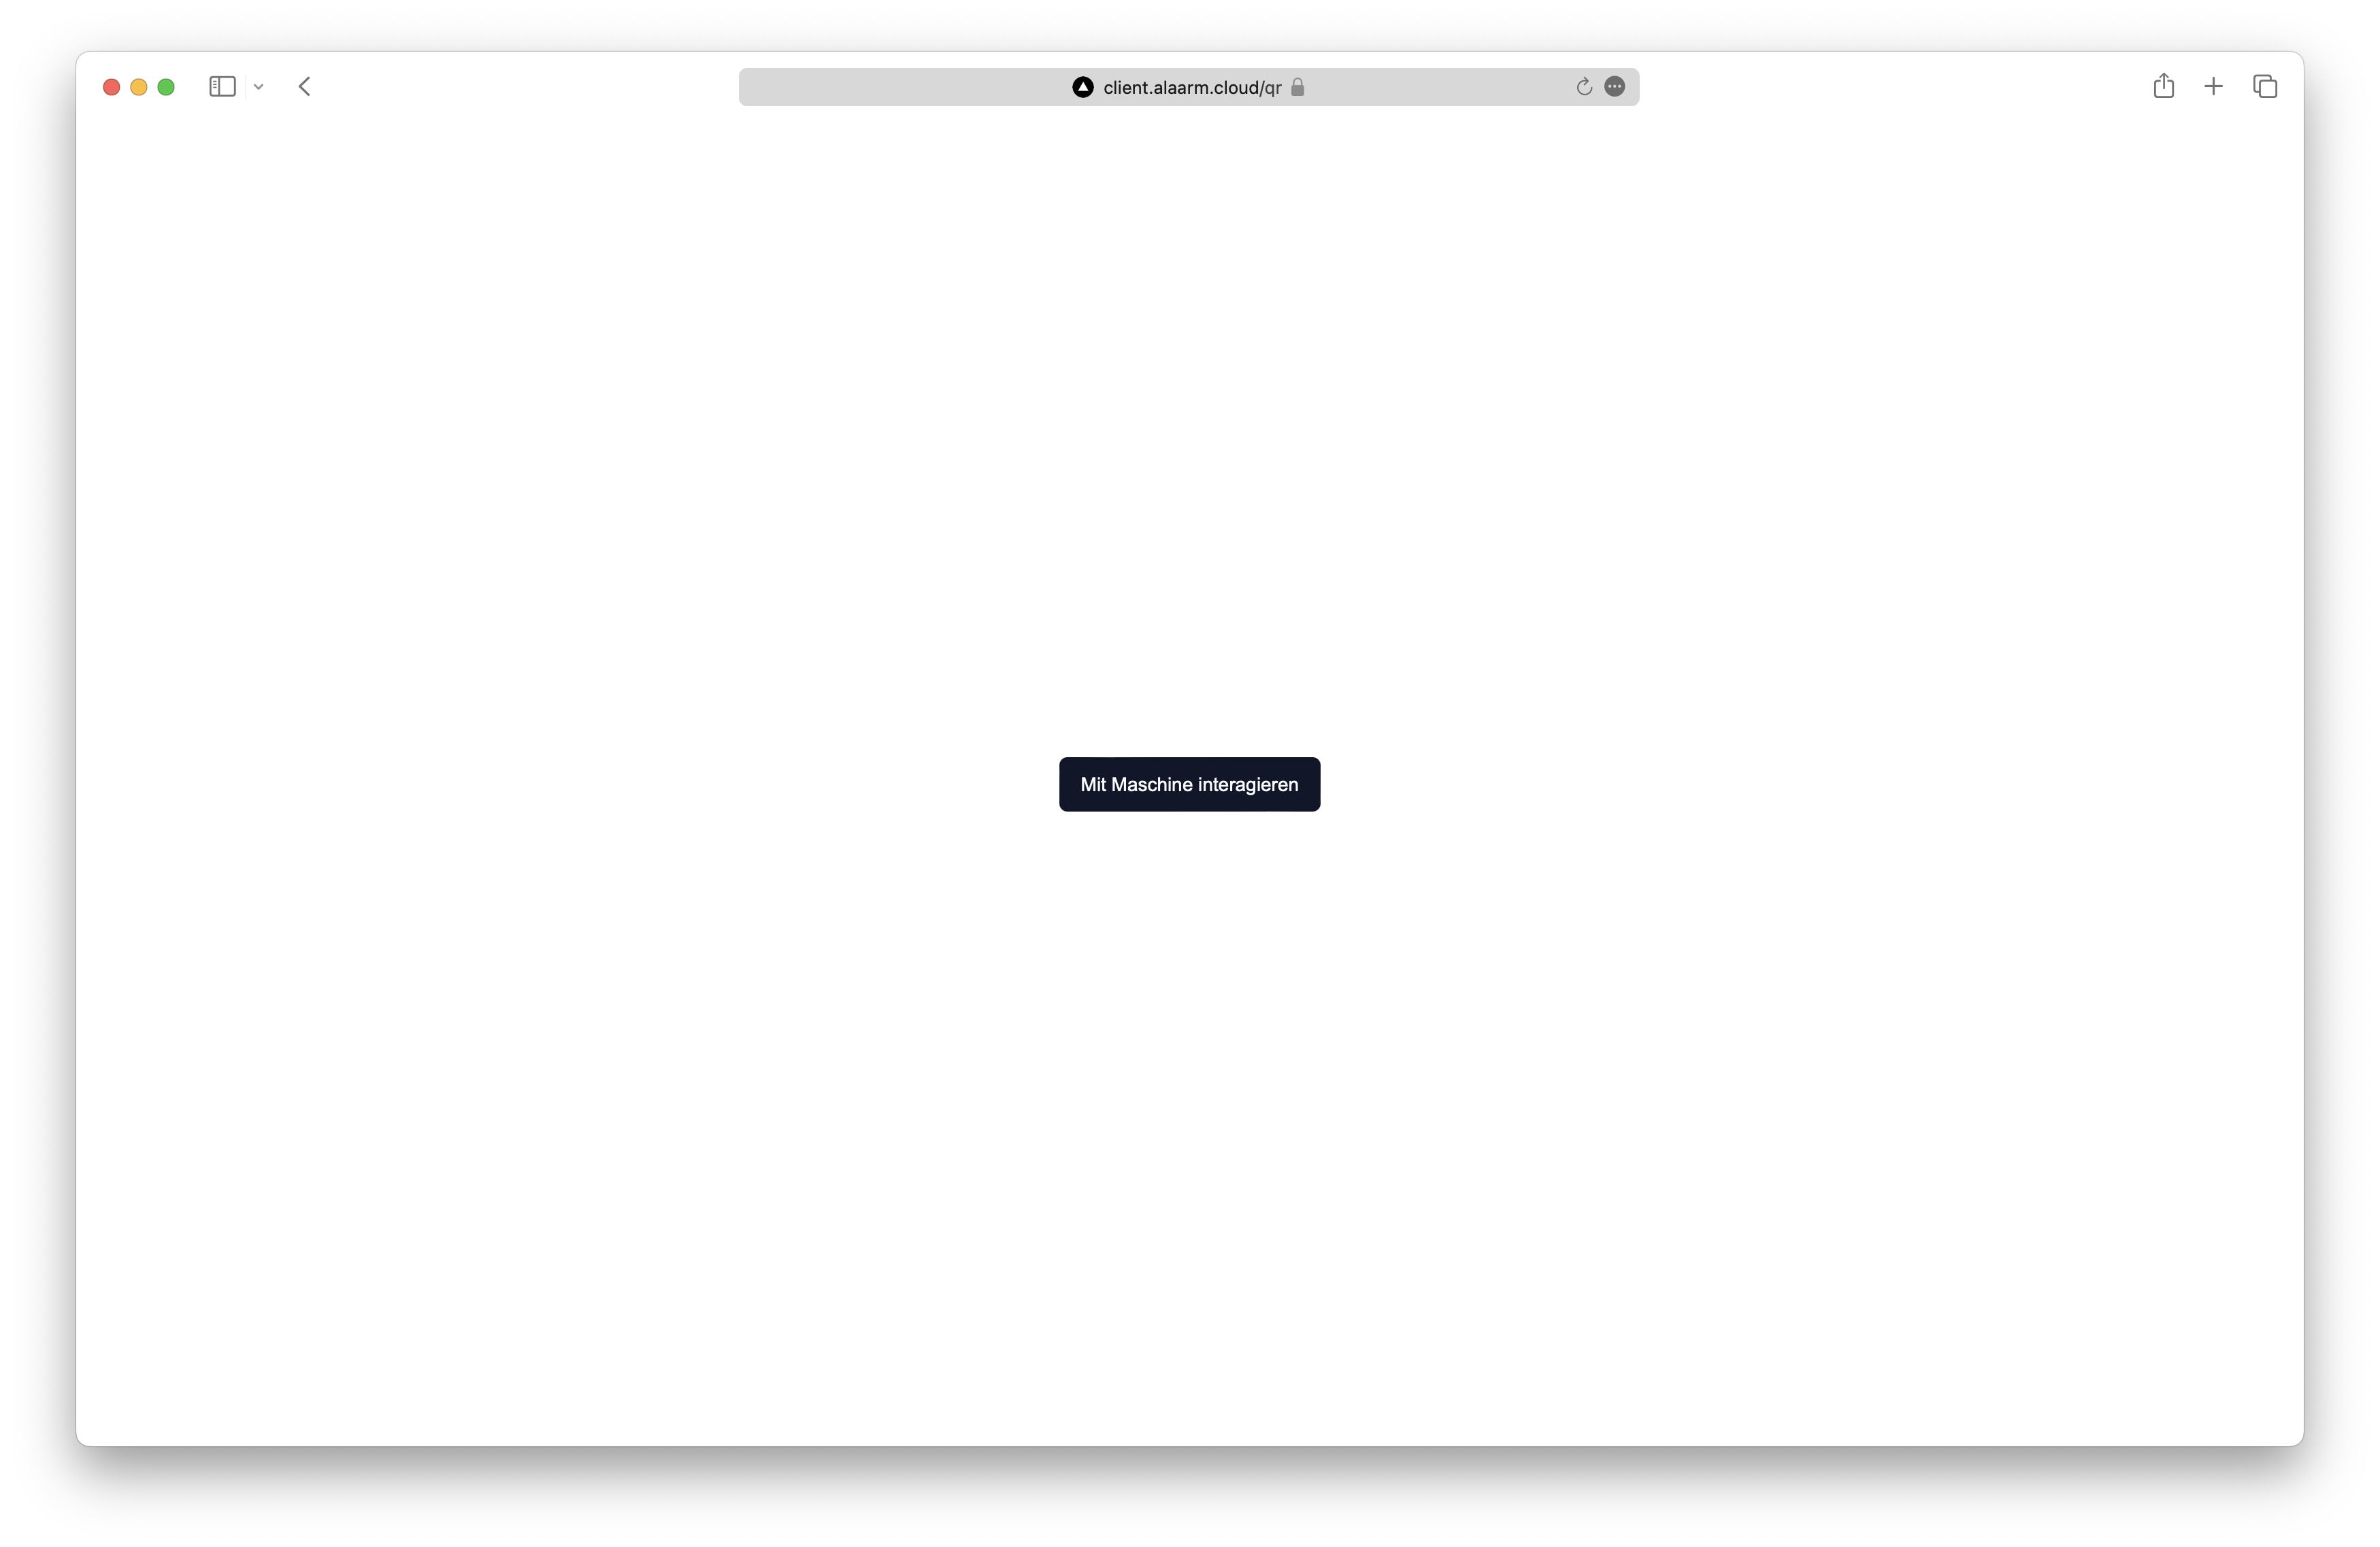
\includegraphics[width=15cm, height=9.61cm]{res/web_interface.png}
    \centering
   \caption{Web Interface}
\end{figure}

Mit der Betätigung des Buttons rollen die Förderbänder der Anlage an. 
Nach Ablauf der konfigurierten Startzeit wird die Eskalationsstufe 1 des Szenarios \textit{Maschinenbrand} ausgelöst. Entsprechende Immersionseffekte werden ausgelöst und die Förderbänder werden gestoppt.

In diesem Moment beginnt für den Übungsteilnehmer der konfigurierte Zeitraum, in dem die aufgetretene Störung zwingend zu lösen ist. Auf der Simulationsoberfläche des Simulationstabletts vom Übungsteilnehmer erscheint ein Fehlercode. Der  Information kann die Person entnehmen, zur welcher Maschine mit dem Störungsbild Brand zu navigieren ist. Auf dem Bildschirm der Maschine ist ein QR-Code eingeblendet, welcher durch den Scanner der Simulationsoberfläche des Simulationstabletts durch den Übungsteilnehmer einzuscannen ist. In der nachfolgenden Abbildung ist die Funktionsweise und der Aufbau des QR Scanners exemplarisch dargestellt:

\begin{figure}[h]
   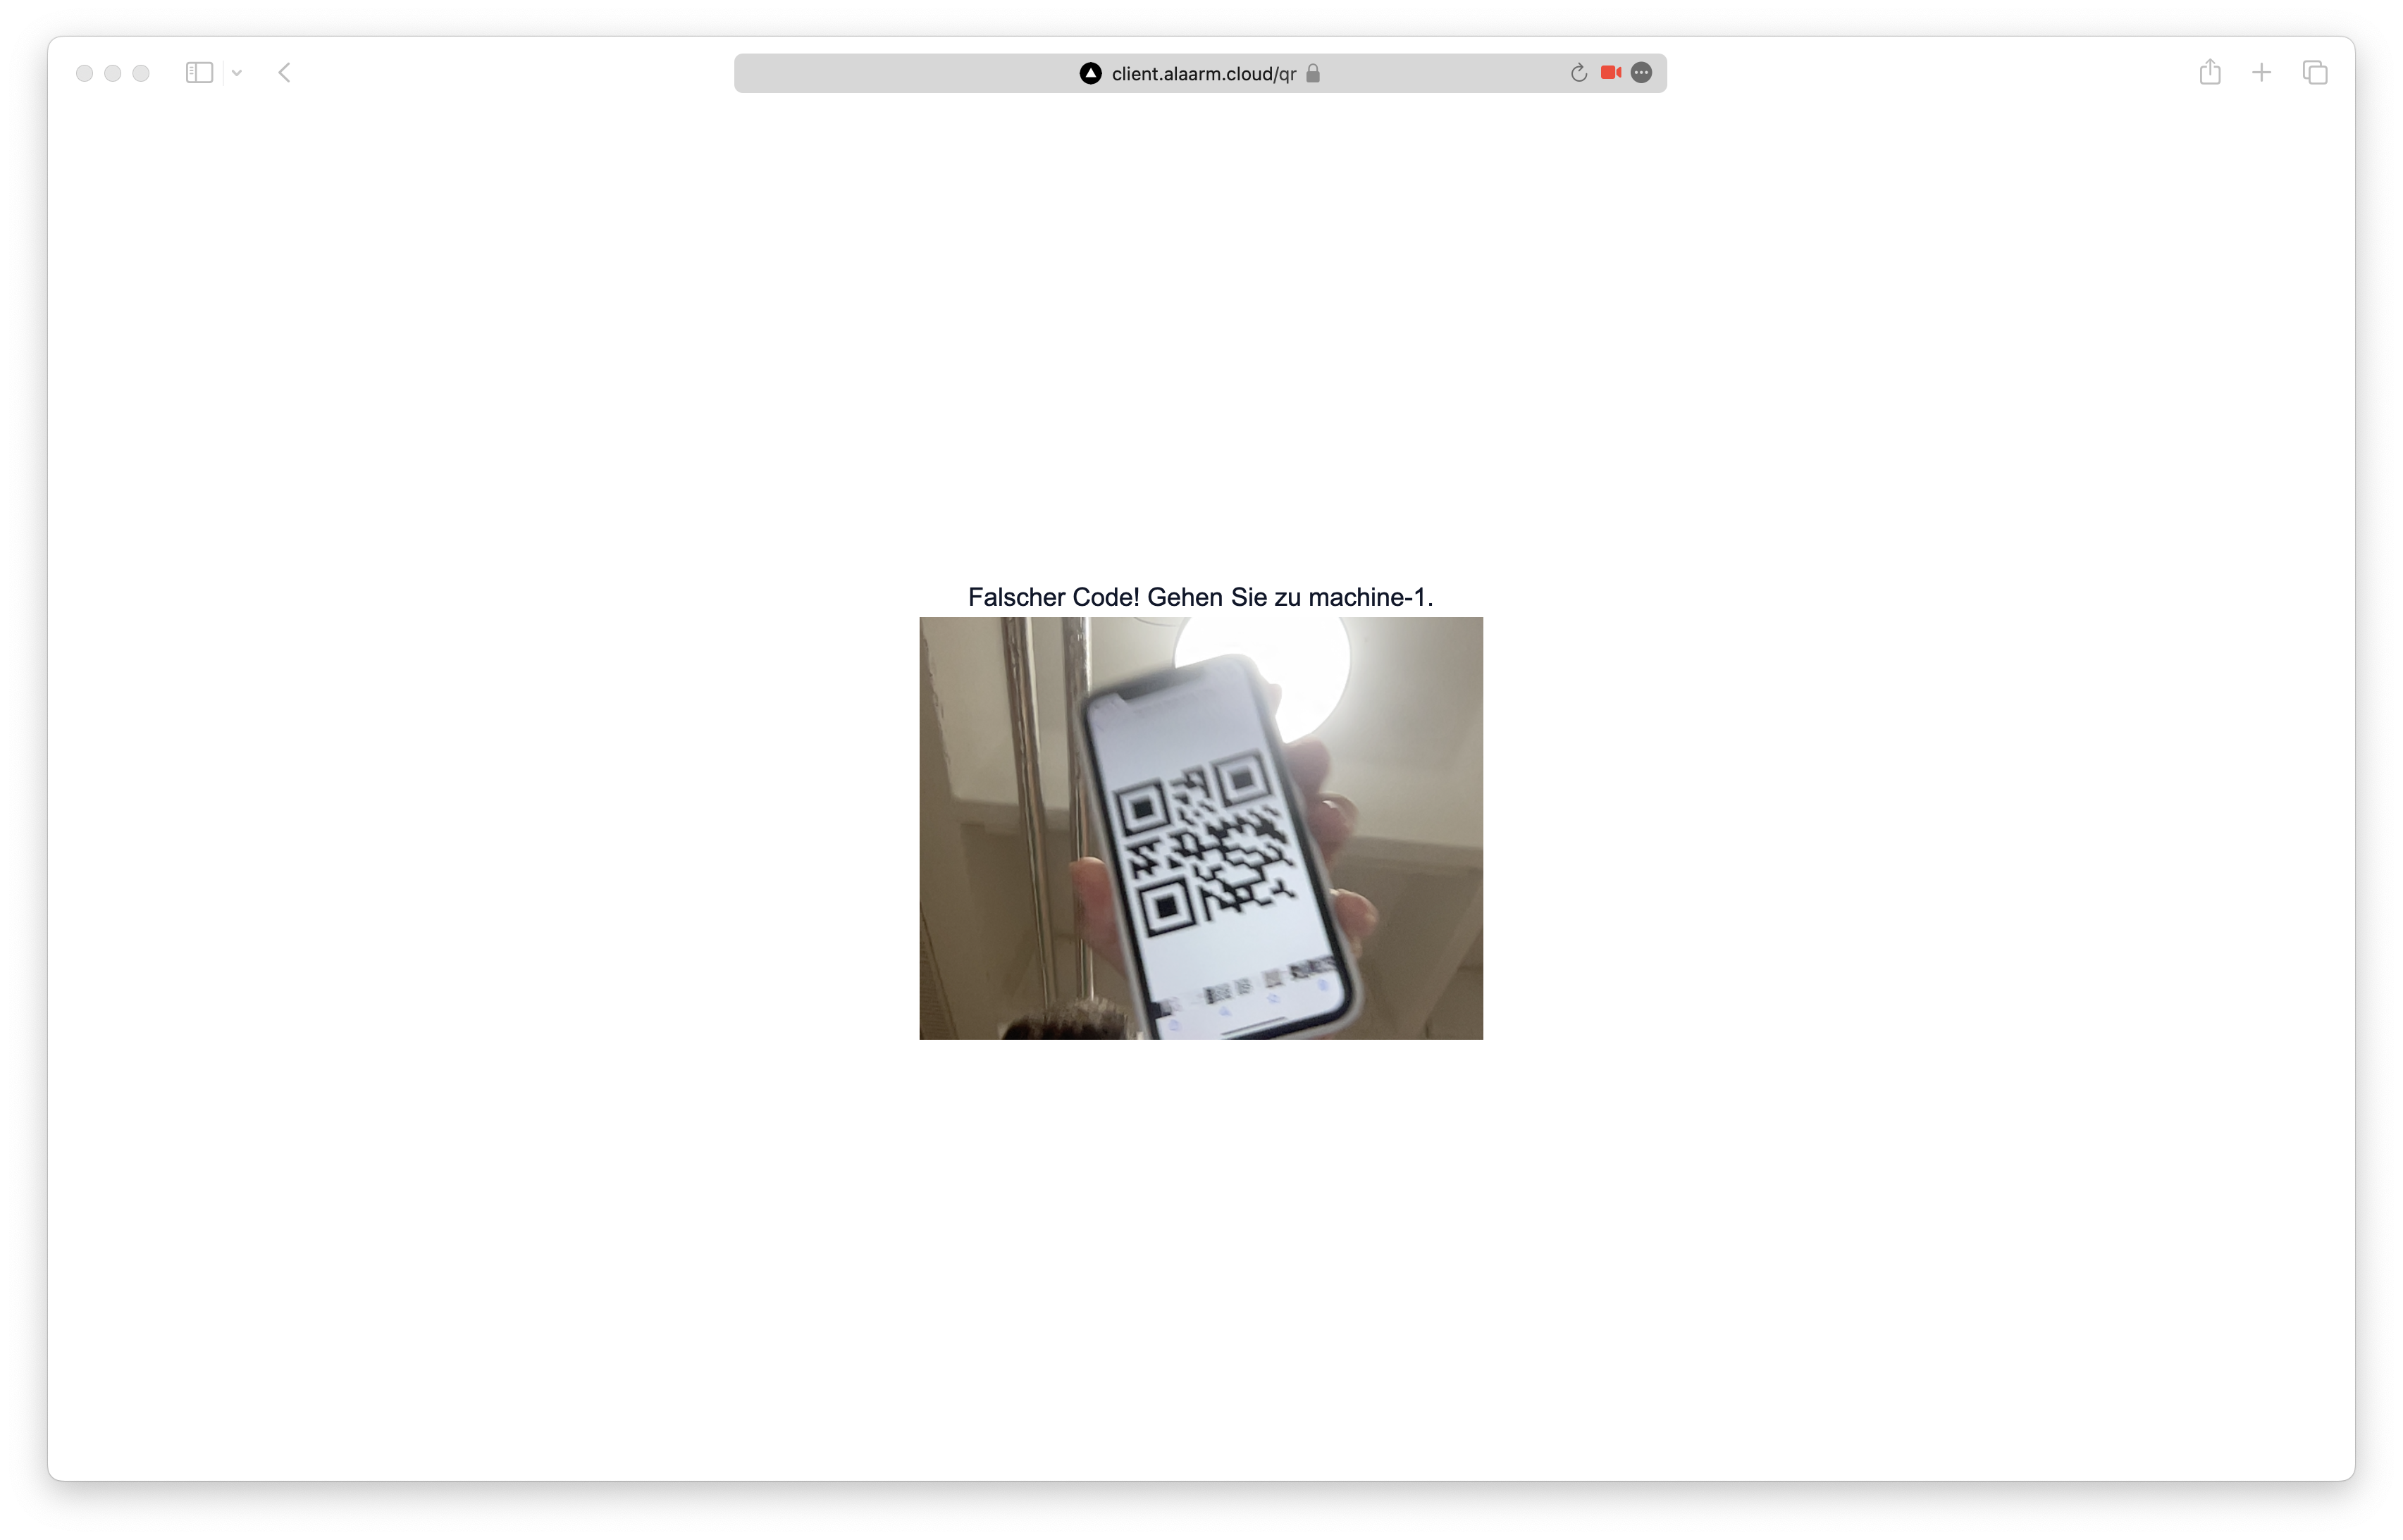
\includegraphics[width=15cm, height=9.61cm]{res/qr_code_scanner.png}
   \caption{QR-Code Scanner}
\end{figure}

Mit dem erfolgreichen Scan beginnt der eigentliche Entstörungsvorgang, für den dem Übungsteilnehmer ein Rätsel zur Entstörung eingeblendet wird. Der Beschreibung des Rätsels ist die Aufgaben zu entnehmen, die der Übungsteilnehmer nun zu lösen hat. Jedes Rätsel zur Entstörung bildet drei Ausgangsszenarien. Sofern das Rätsel falsch gelöst wurde, wird entweder, sofern vorhanden, die nächste Eskalationsstufe mit zusammenhängendem Entstörungsvorgang eingeleitet. Sofern keine weitere Eskalationstufen vorhanden sind, gilt das Alarmszenario für den Übungsteilnehmer als gescheitert. Die zweite Ausgangsmöglichkeit ist die erfolgreiche Lösung des Rätsels zur Entstörung, wobei aufgrund einer durch den Übungsleiter anpassbaren Zufallsvariable bestimmt wird, ob der Entstörungsversuch wirklich erfolgreich war. Sofern die Zufallsvariable für den Übungsteilnehmer ungünstig ist, ist entsprechende Lösung nicht ausreichend für die Behebung und ggf. wird eine weitere Eskalationsstufe eingeleitet. Sofern die Zufallsvariable sich nicht der erfolgreichen Lösung des Entstörungsvorgangs entgegenstellt, ist ein erfolgreicher Entstörungsversuch und damit eine erfolgreiche Beendigung des Alarmszenarios nur gegeben, wenn der Zeitraum zur Lösung der Entstörung eingehalten wurde. Ist dies nicht der Fall, werden bei Verfügbarkeit weitere Eskalationsstufen eingeleitet oder das Szenario gilt auch hier als gescheitert.  

\subsubsection{Eskalationsstufen}

Das realisierte Szenario \textit{Maschinenbrand} verfügt über insgesamt drei Eskalationsstufen.

Bei der \textbf{ersten Eskalationsstufe} werden als Immersionsobjekte der Lautsprecher, Subwoofer und die Andon-Signalleuchte adressiert. Vom Lautsprecher und Subwoofer wird ein leiser, langsamer und leicht pulsierender Sound des Knackens und Rauschens abgespielt. Gleichzeitig schaltet sich die rote Lampe der Andon-Lampe an, um eine Störung der Maschine zu signalisieren.

Im Rahmen der \textbf{zweiten Eskalationsstufe} wird durch die Lautsprecher und den Subwoofer ein schnellerer, stärker pulsierender Sound mit ähnlichen Geräuschen abgespielt. Zusätzlich wird Brandduft über einen Vaporizer ausgesondert und eine LED innerhalb der Maschine fängt an mit blauem Licht zu flackern. 

Bei der letzten, \textbf{dritten Eskalationsstufe} des \textit{MVP} Szenarios beschleunigt sich der Sound des Brandgeräusches, der durch den Lautsprecher und Subwoofer abgespielt wird. Dazu wird verstärkt Brandgeruch und Rauch durch den Vaporizer ausgesondert. Der LED-Streifen in der Maschine beginnt nun rot zu flackern, um Flammen zu imitieren. Zusätzlich wird eine Wärmelampe angesteuert, welche zur Emittierung von Wärme aktiviert wird.

Durch den stufenbasierten Aktivierungslauf, sofern der Entstörungsvorgang nicht erfolgreich durch den Übungsteilnehmer absolviert wird, kann die immersive Wahrnehmung des Alarmszenarios des Übungsteilnehmers im Zeitverlauf gesteigert werden. Mithilfe der gewählten Konfiguration kann ein reales Szenario des Maschinenbrandes und die Effekte auf Maschinenführer simuliert werden. Die Ablauflogik kann als Überblick im Kapitel \ref{chap:process model} visuell nachvollzogen werden.

\subsubsection{Entstörungsvorgänge}

An jede aktivierte Eskalationsstufe schließt ein individueller Entstörungsvorgang an. Der Übungsteilnehmer bekommt bei Auslösung einer Eskalationsstufe einen Fehlercode übergeben, auf Basis dessen Informationen die richtige Maschine anzulaufen ist. Via Scan des QR-Codes an der Maschine wird die Oberfläche zur Entstörung aufgerufen. Je nach Eskalationsstufe im \textit{MVP}-Szenario wird eines von insgesamt drei Rätseln aufgerufen.

Der \textbf{erste Entstörungsvorgang} des MVPs gibt dem Übungsteilnehmer den Hinweis, dass aufgrund des \textit{Fehlers E5432} der Betriebsablauf der Anlage im \textit{Zentrum Industrie 4.0} gestört ist. Um die Reihenfolge an Werkschritten wiederherzustellen, müssen auf der Weboberfläche des Tablets des Endnutzers die Nummern 1 bis 10 in aufsteigender Reihenfolge angewählt werden. Initial ist eine Zeitbegrenzung von 10 Sekunden vorgesehen. Die Strukturierung von Rätseln kann anhand der nachfolgenden Abbildungen nachvollzogen werden.

\begin{figure}[H]
   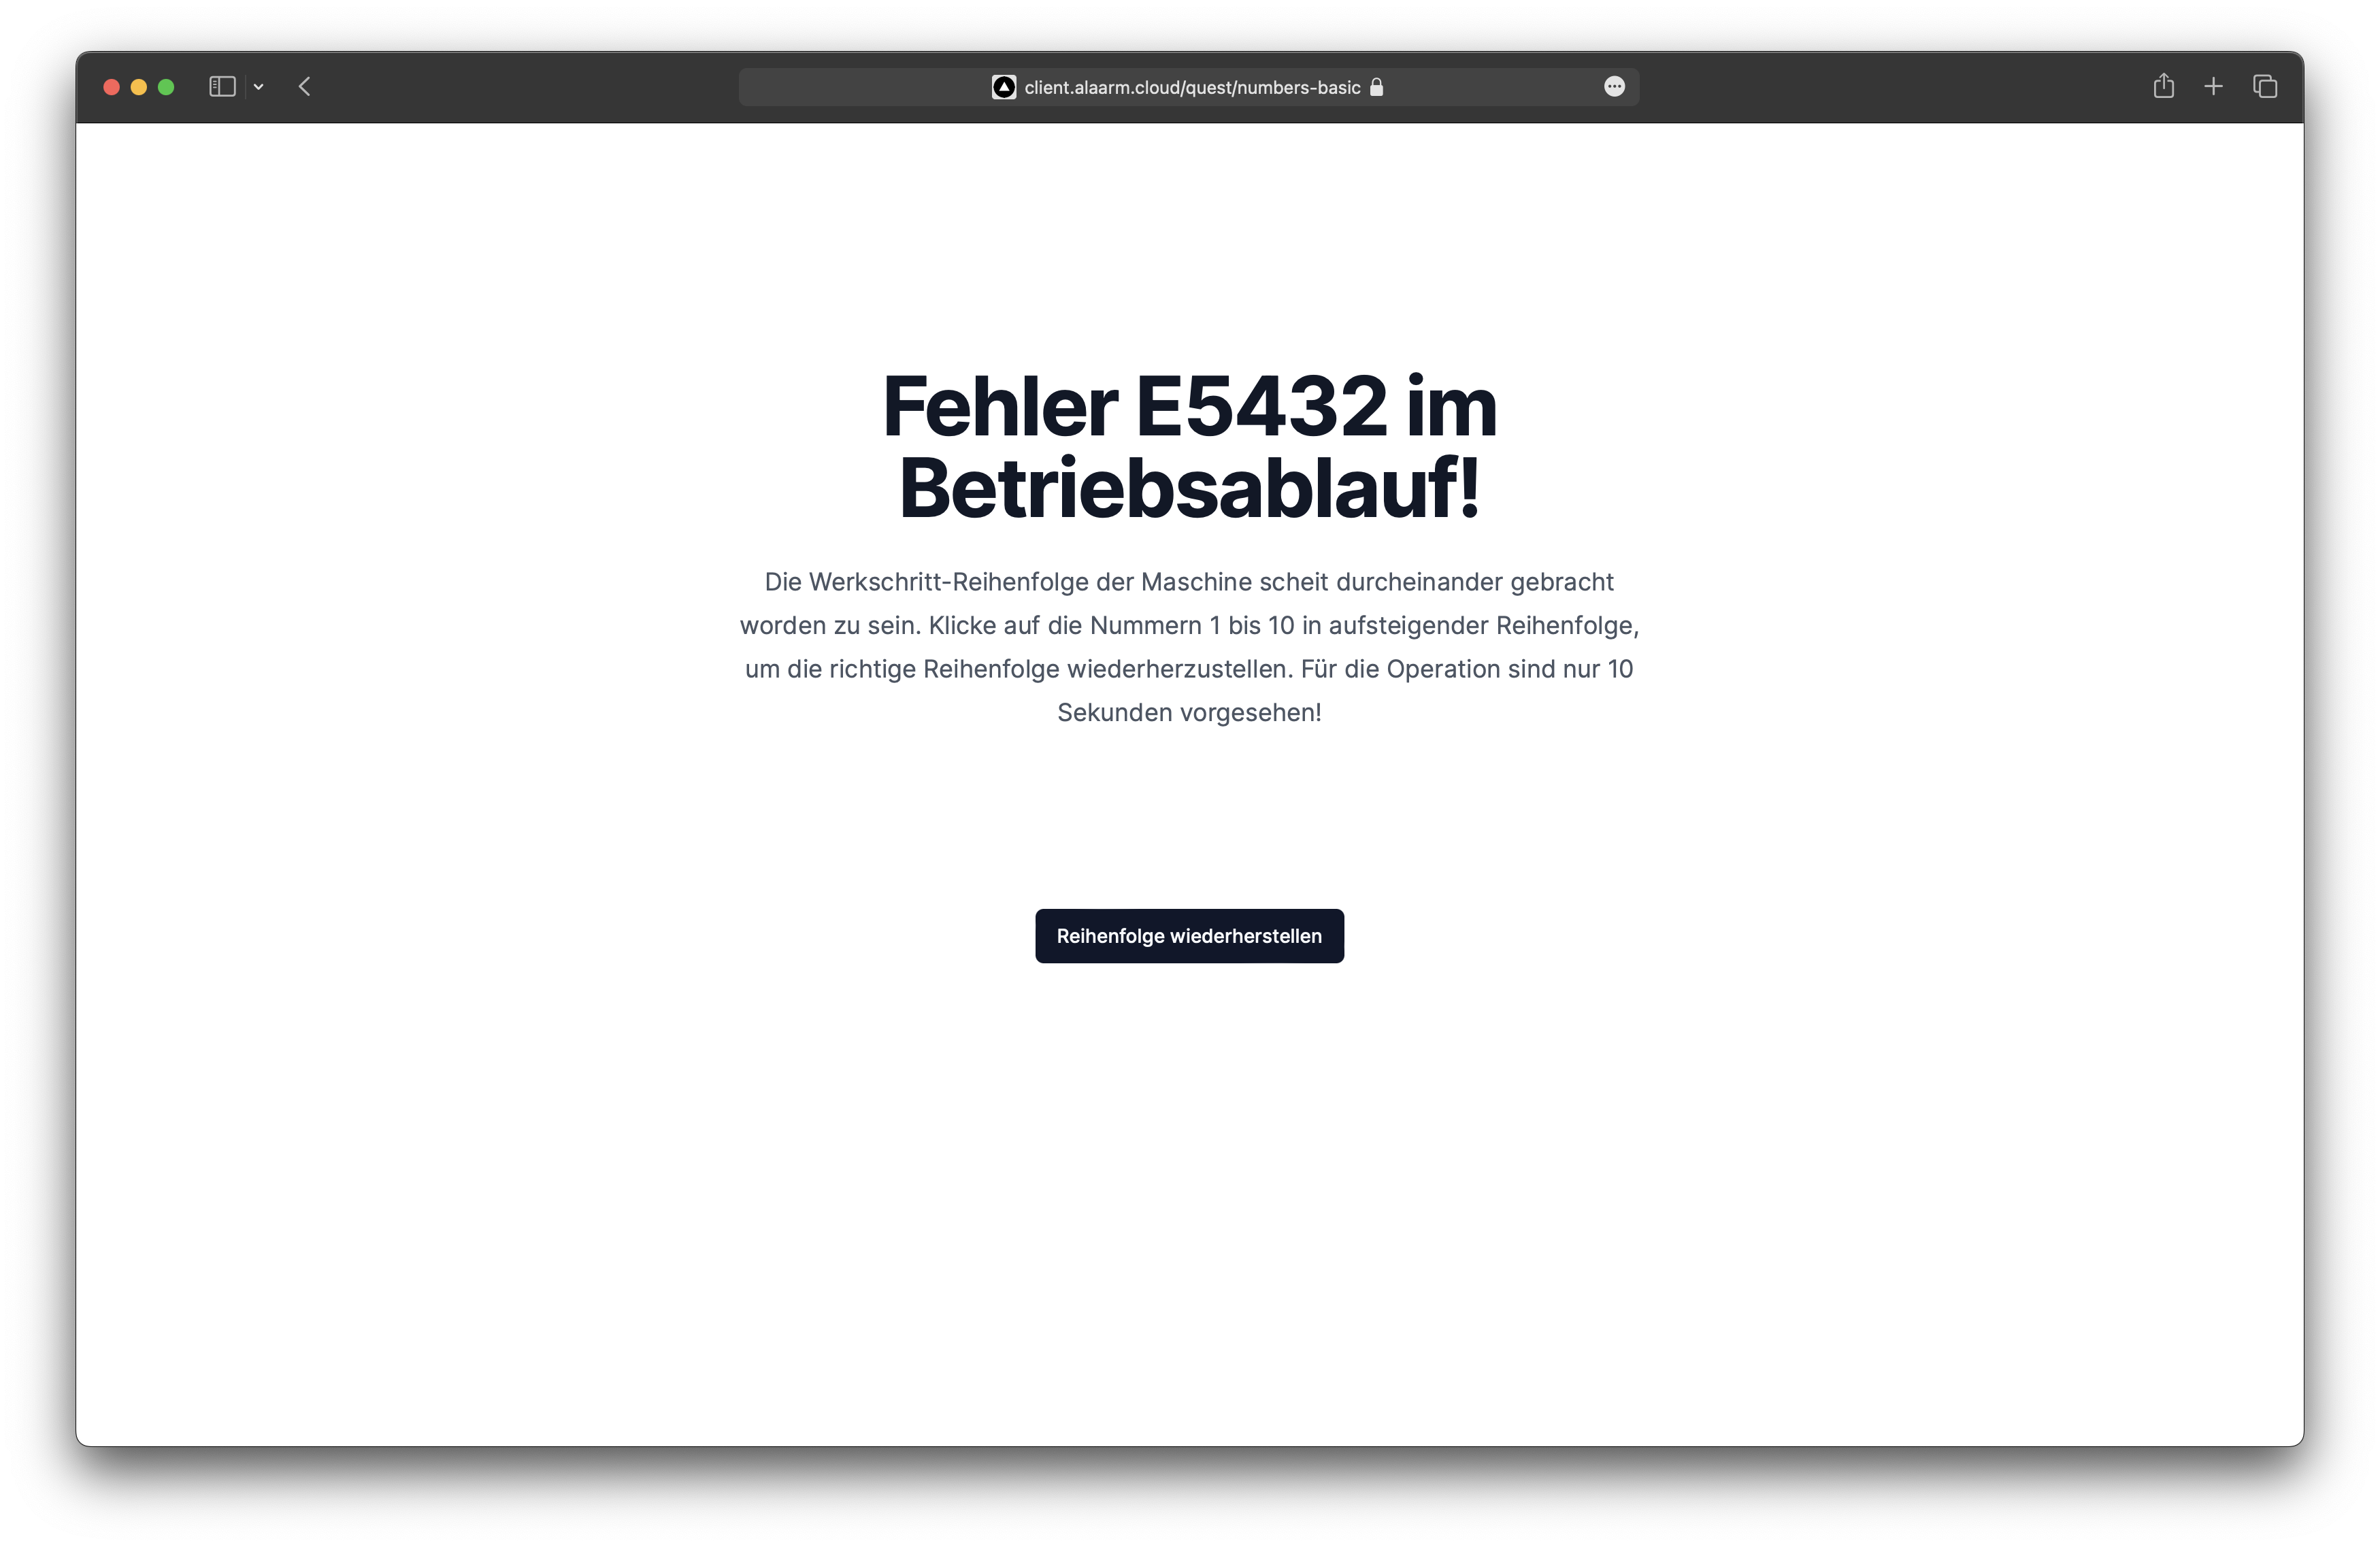
\includegraphics[width=15cm, height=9.61cm]{res/quest_01_v2.png}
   \caption{Hinweisseite - Rätsel 1}
\end{figure}

\begin{figure}[H]
   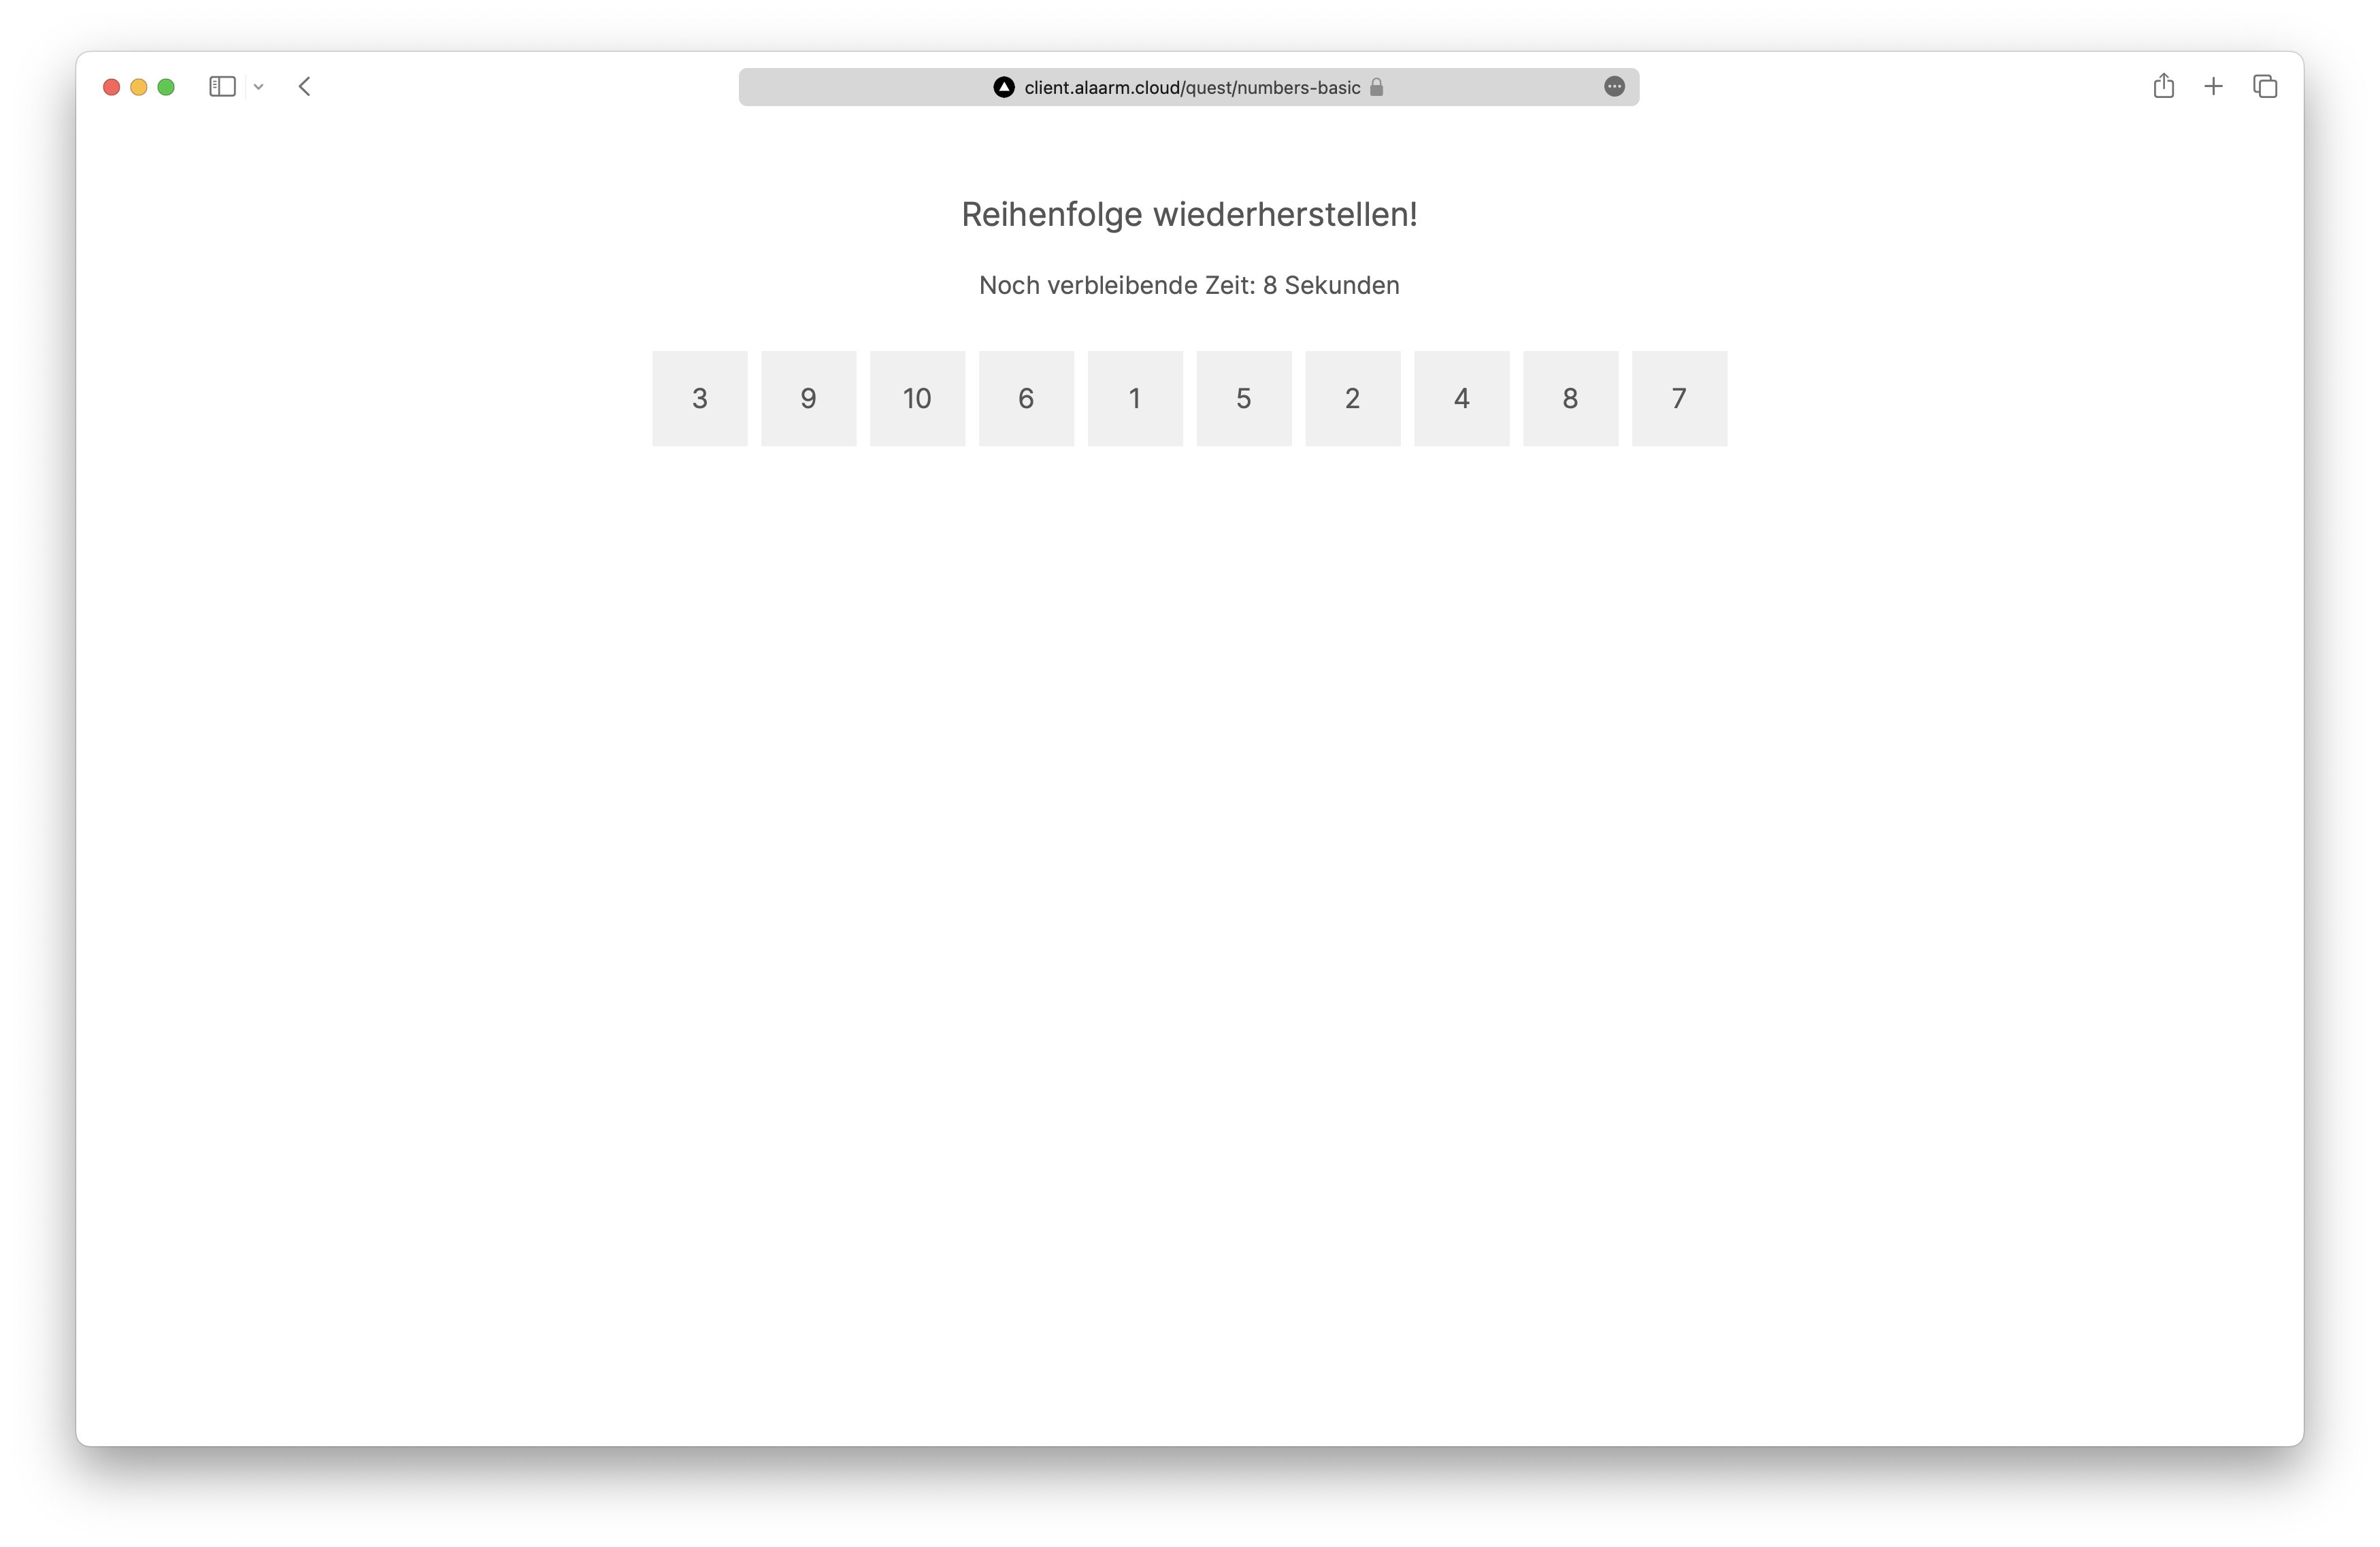
\includegraphics[width=15cm, height=9.61cm]{res/quest_01.png}
   \caption{Rätsel 1}
\end{figure}

Sofern es zum \textbf{zweiten Entstörungsvorgang} kommt, ist ein Rätsel mit dem Störungsbild \textit{P4222 - Störung des Produktionsprozesses} zu lösen. Hier ist eine Störung im Prozessfluss der Maschine gegeben, wodurch es zur Alarmlage der Überhitzung kommt. Auch hier müssen Prozesse in die richtige Reihenfolge gebracht werden, wobei die Prozessschritte durch eine Neukalibrierung nach 5 und 10 Sekunden neu gemischt werden. Die graphische Realisierung kann der nachgelagerten Grafik entnommen werden:

\begin{figure}[H]
   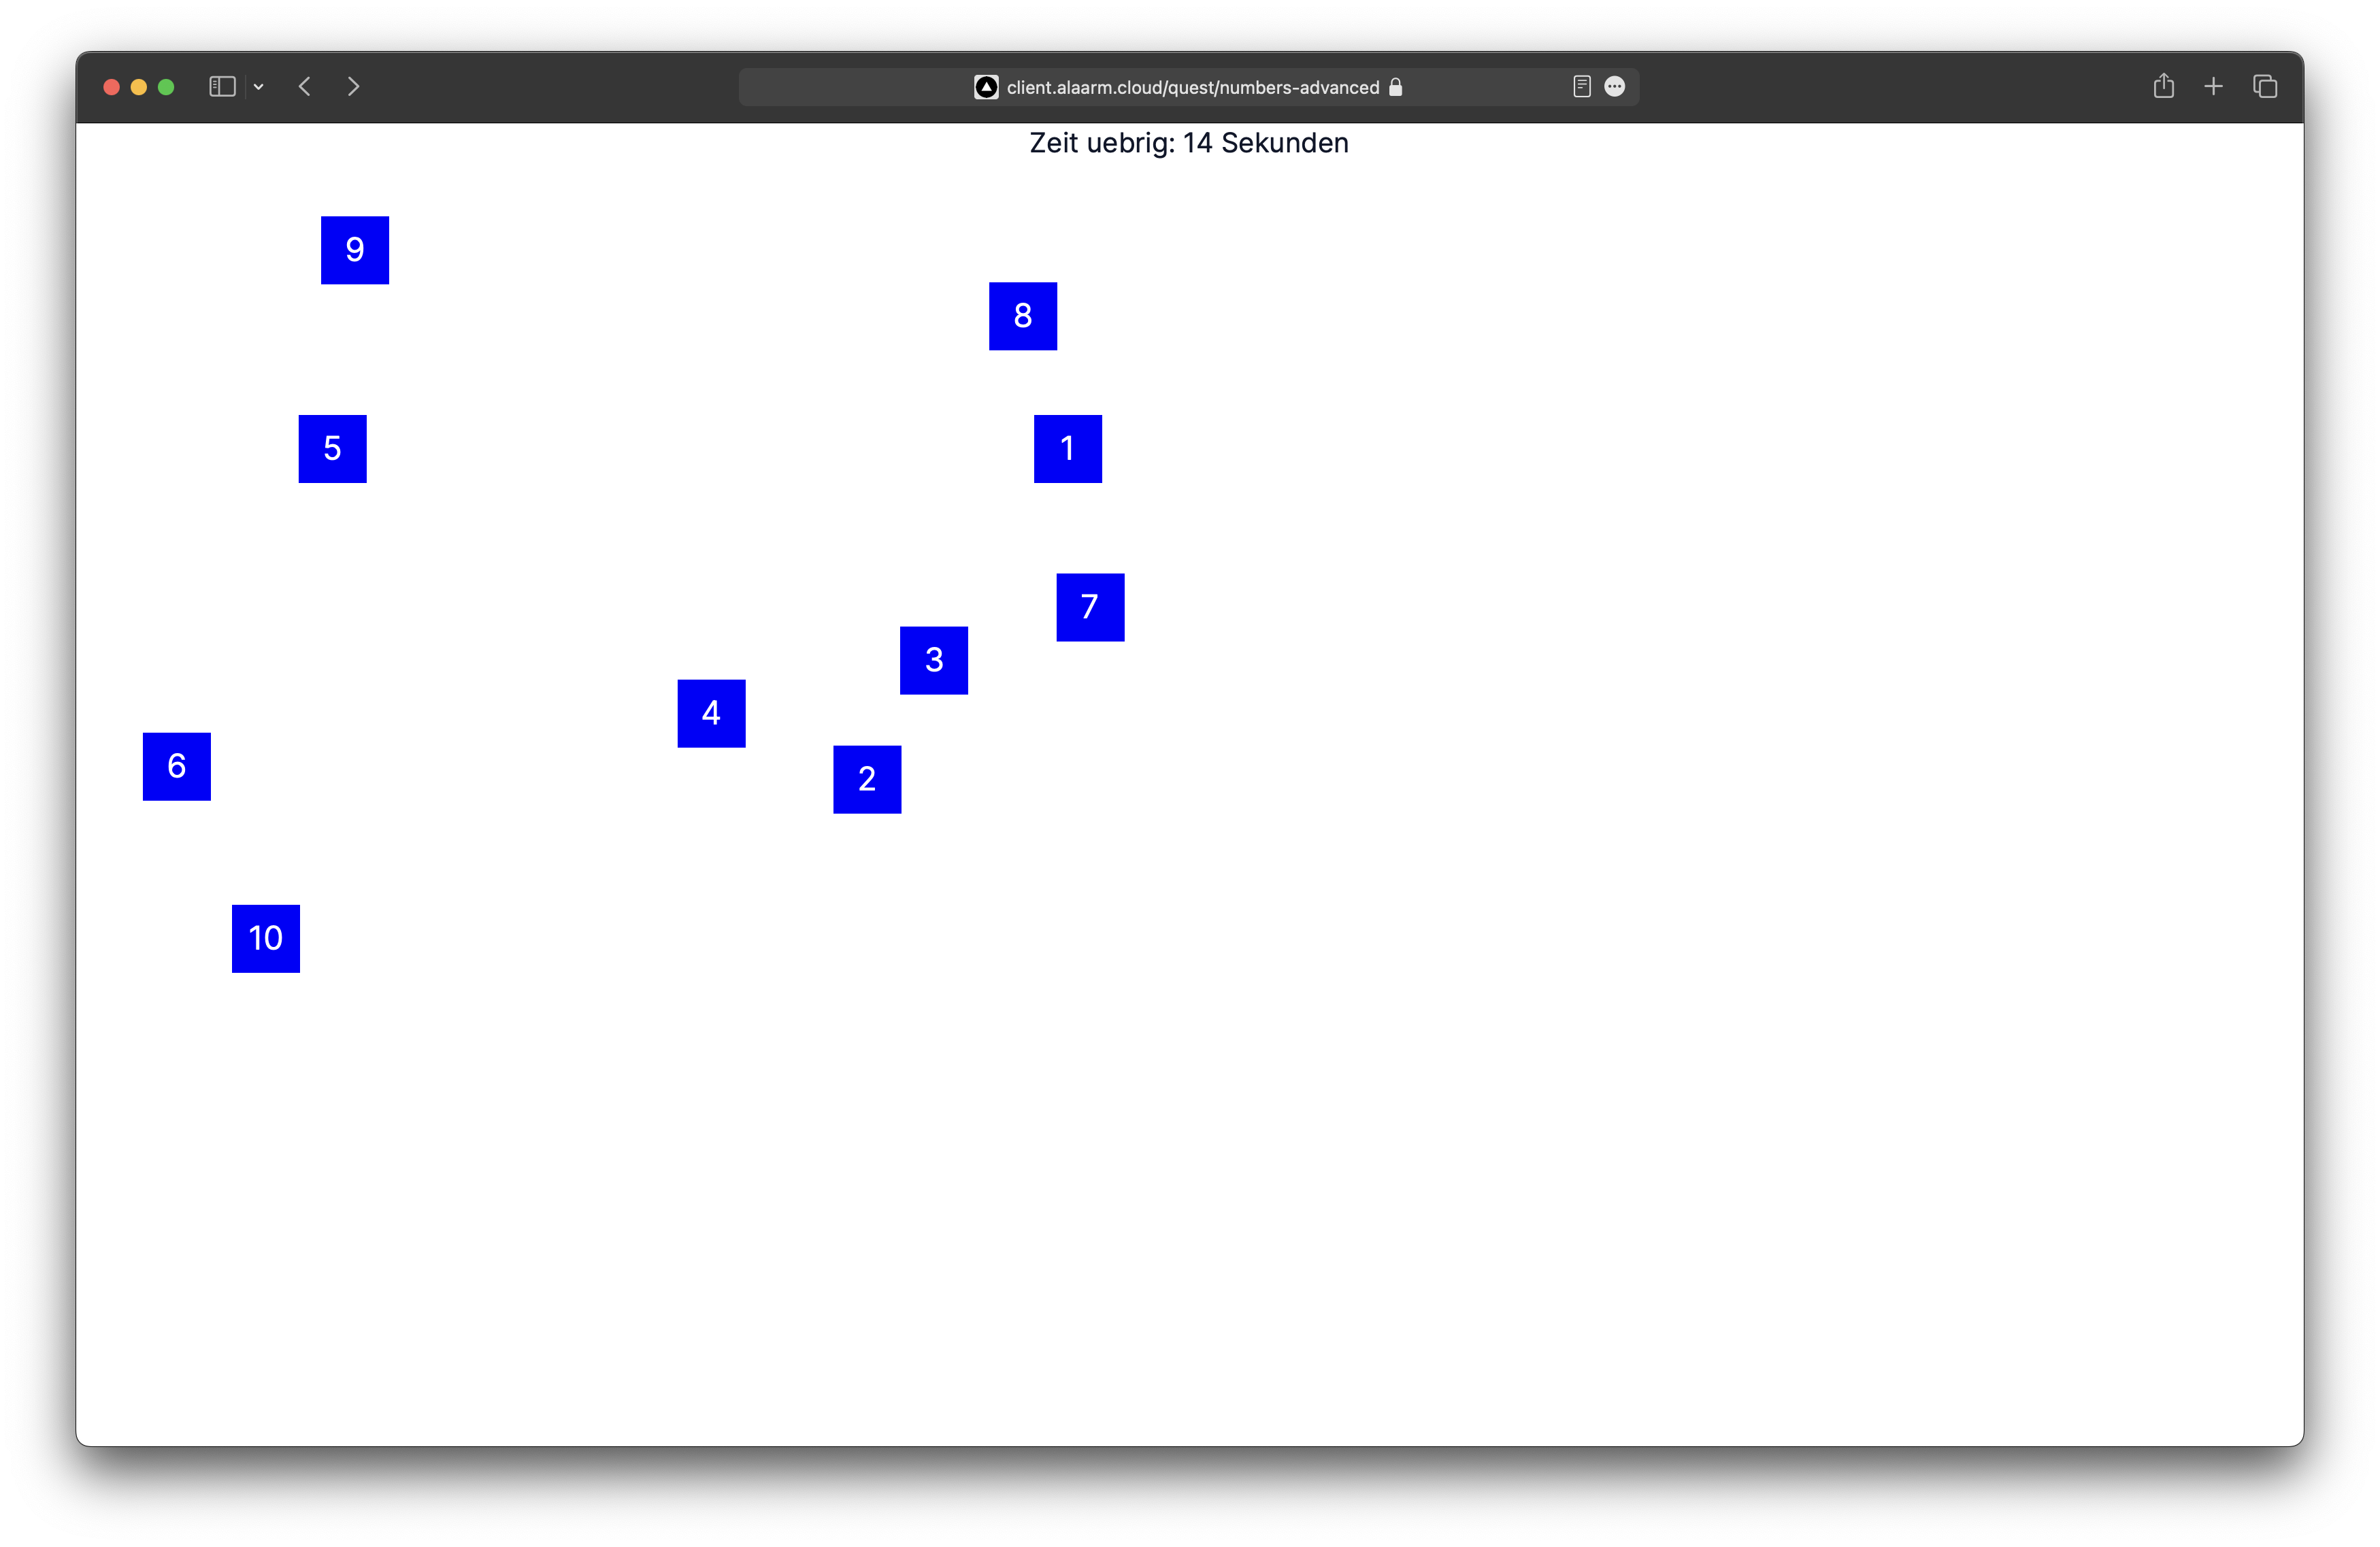
\includegraphics[width=15cm, height=9.61cm]{res/quest_02.png}
   \caption{Rätsel 2}
\end{figure}

In dem potentiell letzten, \textbf{dritten Störungsvorgang} des MVPs \textit{Problem K1213 mit der Kalibrierung} ist ein schwerwiegendes Fehlerbild in der Kalibrierung der Maschine zu beheben. Durch eine Fehlkalibrierung ist es zu einem Kabelbrand gekommen. Um den Schaden zu begrenzen, müssen die Eingaben schnellstmöglich neu kalibriert werden, um einen Brand zu verhindern. Zur korrekten Kalibrierung muss ein grün aufleuchtender Bereich auf der Weboberfläche des Übungsteilnehmers innerhalb von 0,6 Sekunden gedrückt werden. Der Bereich ist dabei initial schwarz gefärbt. Im Falle einer rechtzeitigen Reaktion ist die Maschine kalibriert, eine Ausweitung des Brandes abgewandt und das Szenario erfolgreich beendet. Das Kalibrierungsrätsel ist folgender Abbildung zu entnehmen:

\begin{figure}[H]
   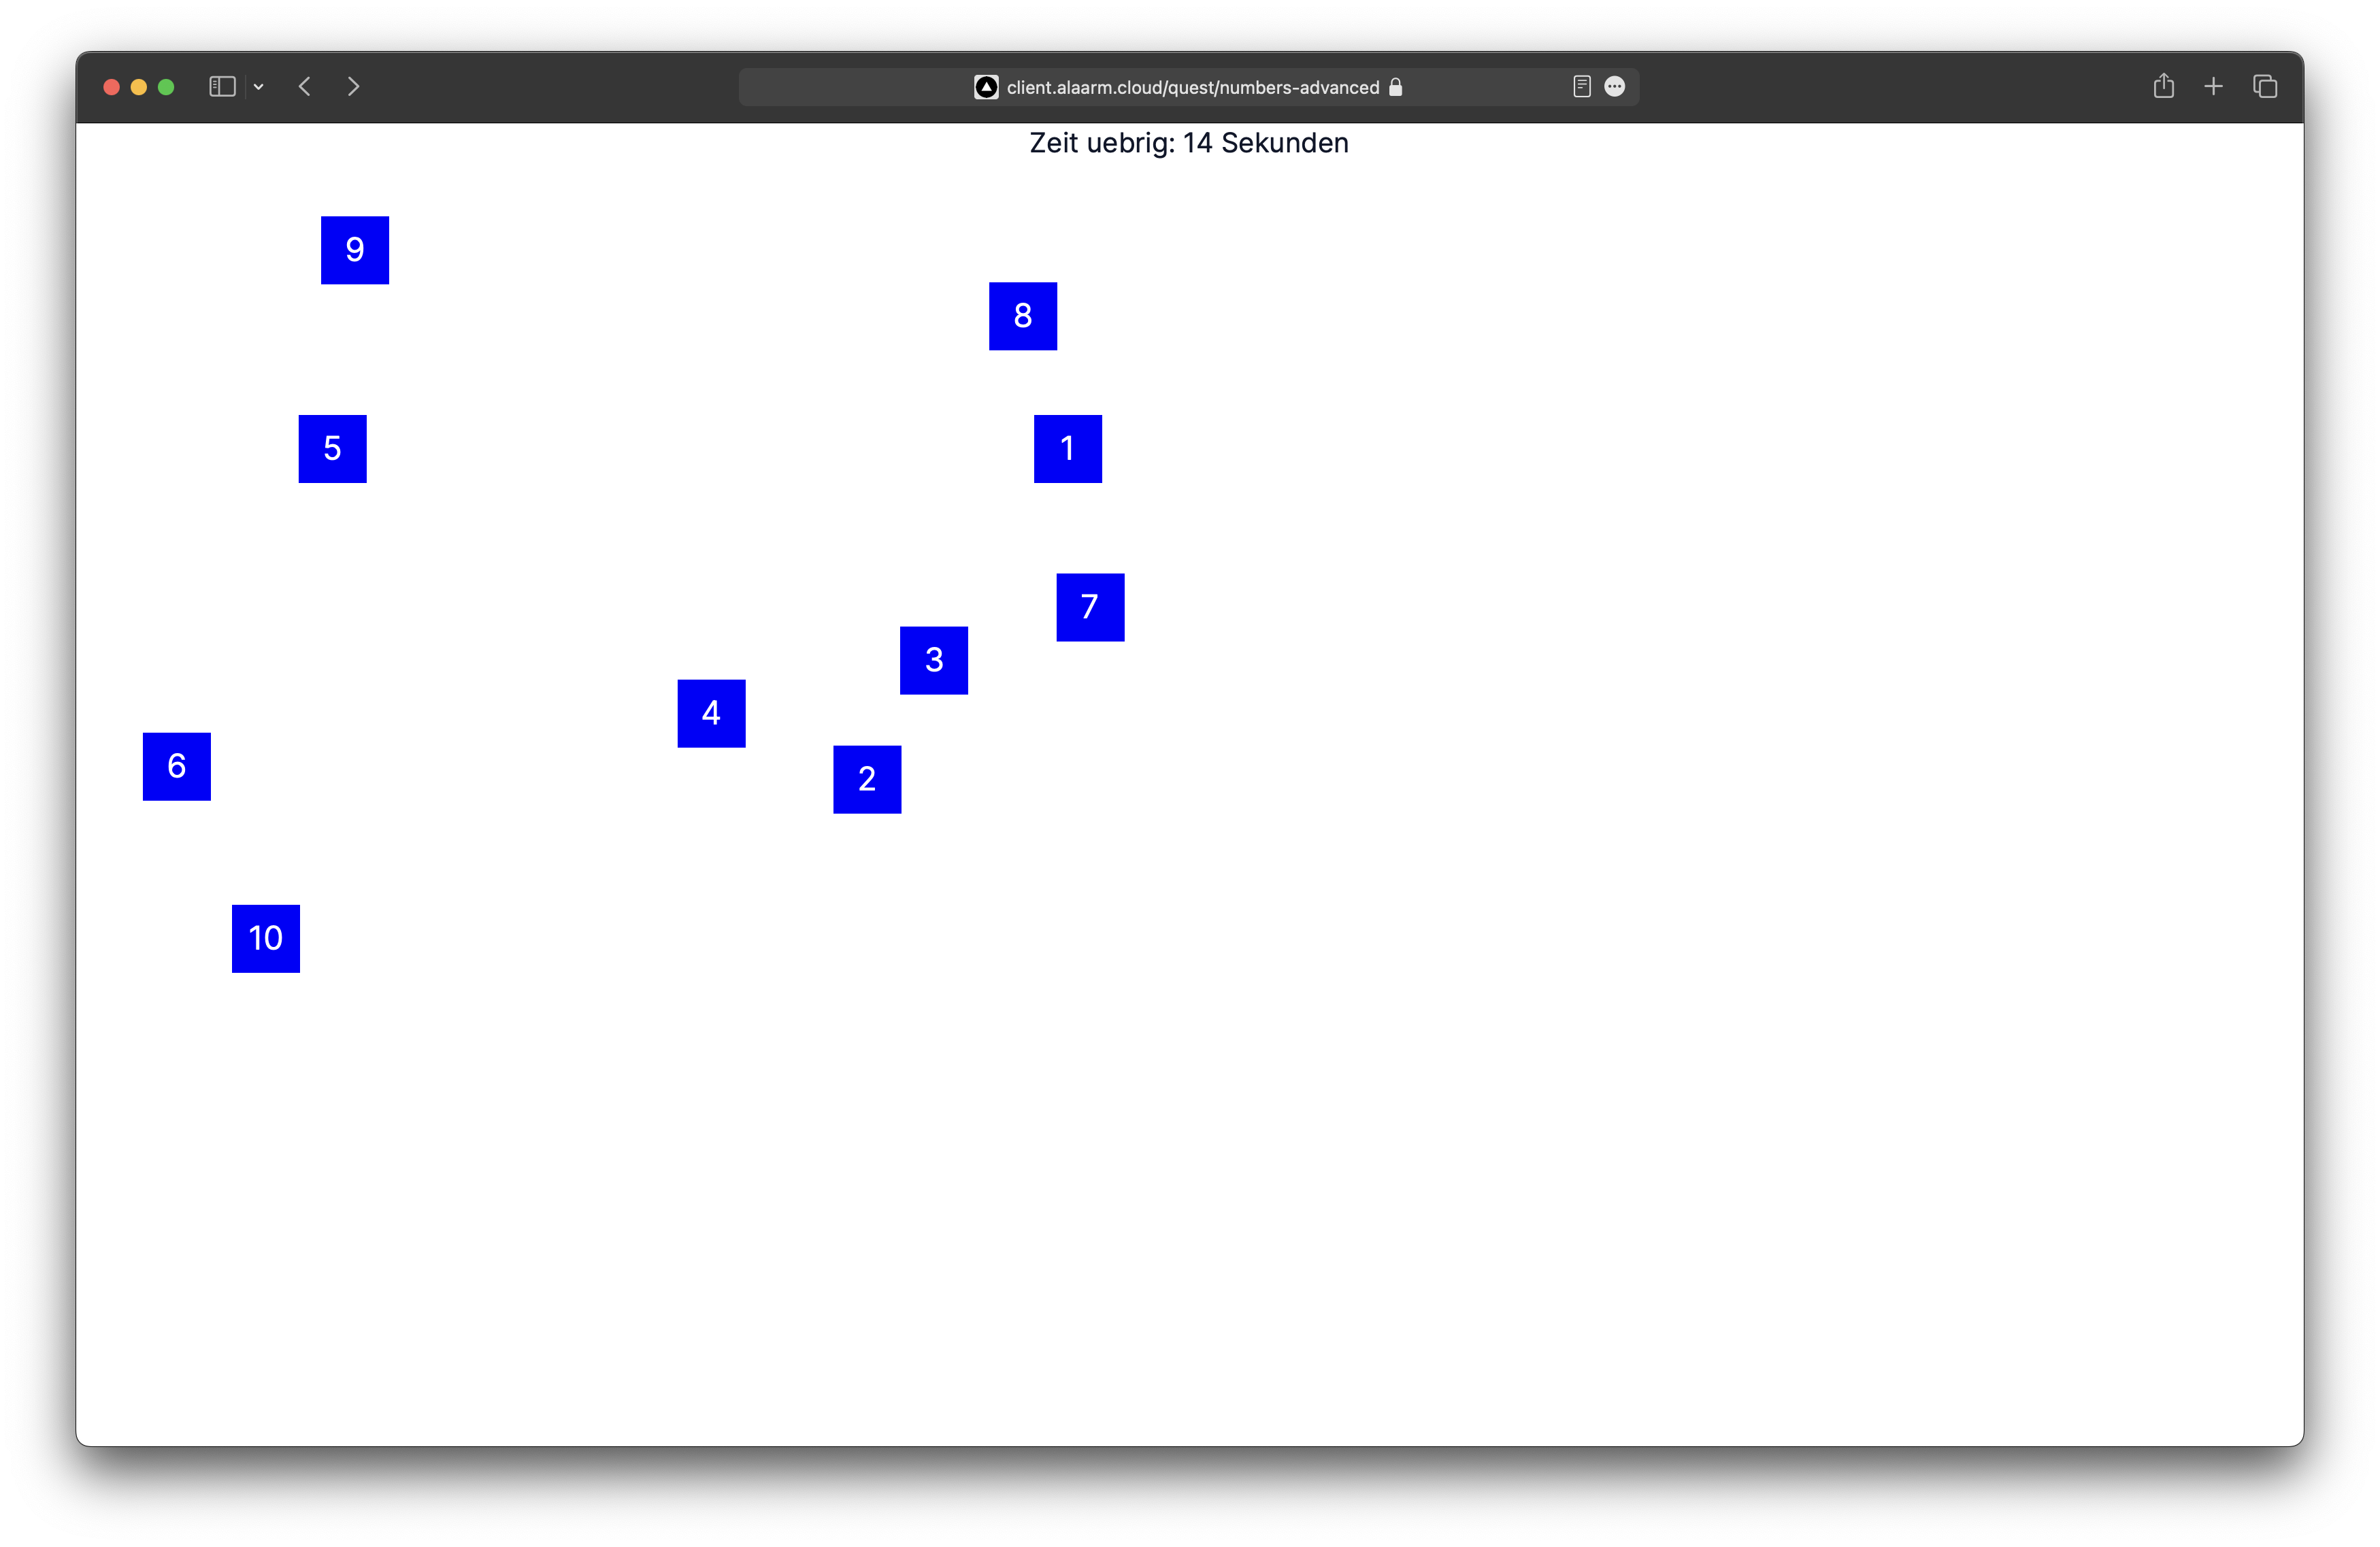
\includegraphics[width=15cm, height=9.61cm]{res/quest_02.png}
   \caption{Rätsel 3}
\end{figure}

\subsubsection{Administration der Alarmsimulation}

Die Verantwortung und Steuerung der Alarmsimulation wird durch den Übungsleiter getragen. Neben dem Start der Simulation kann auf einer Web-Oberfläche des Admintablets das Szenario individuell konfiguriert werden. Beispielsweise können Anpassungen wie veränderte Sounddateien, weitere Eskalationsstufen, Zufallsvariablen für die Erfolgswahrscheinlichkeit einer Entstörung und Zeiträume zur Lösung einer Eskalationsstufe definiert werden.

\subsection{Begleitende Dokumente}
\usepackage{hyperref} 
Für die Simulation wurde eine generelle Bedienungsanleitung und ein Sicherheitsbriefingbogen entworfen, um den Übungsleiter bei der Anleitung von neuen Übungsteilnehmern zu unterstützen. Jene Dokumente können dem \hyperref[sec:anhang]{Anhang} entnommen werden.

\begin{comment}
\subsection{Sicherheitsbriefing}\hspace{0pt}\marginpar{\footnotesize{ca. 2 Min.}}

\emph{Bitte nehmen Sie sich die Zeit, diese Anweisungen sorgfältig zu lesen und zu verstehen, bevor Sie mit dem Betrieb der Maschine fortfahren. Ihre Sicherheit hat oberste Priorität.}

\newpage

\emph{WICHTIG: GESUNDHEITSWARNUNG \\
Bitte stellen Sie sicher, dass Sie die geeignete Schutzkleidung tragen, bevor Sie mit dem Betrieb dieser Maschine beginnen. Dies beinhaltet Schutzhandschuhe, Schutzbrille und Atemschutzmaske. Bitte entnehmen Sie die Schutzkleidung, die rechts von Ihnen liegt. 
Es besteht die Möglichkeit, dass während des Szenarios Rauch oder andere intensiv riechende Substanzen verwendet werden.
Dieses Szenario beinhaltet flackernde Lichter, die bei einigen Personen mit Epilepsie zu Anfällen führen können. 
Bitte beachten Sie, dass Ihre Gesundheit und Sicherheit oberste Priorität haben. Falls Sie Bedenken haben oder gesundheitliche Einschränkungen haben, die sich auf Ihre Teilnahme an diesem Szenario auswirken könnten, empfehlen wir Ihnen, vorab Rücksprache mit einem Arzt zu halten, um sicherzustellen, dass Sie angemessen geschützt sind und das Szenario ohne Risiken für Ihre Gesundheit durchführen können.}

\

\subsection{Bedienungsanleitung und Aktivierung der Eskalationsstufe}
\

\emph{BEDIENUNGSANLEITUNG \\
1.	Überprüfen Sie, ob alle Sicherheitsvorkehrungen getroffen wurden und die Maschine bereit für den Betrieb ist. \\
2.	Drücken Sie den grünen Startknopf auf der rechten Seite des Bedienfelds, um den Maschinenprozess zu starten. \\
3.	Überwachen Sie den Prozess auf dem Bildschirm. Achten Sie auf alle Warnungen oder Fehlermeldungen, die angezeigt werden könnten. \\
4.	Im Falle einer Fehlermeldung, drücken Sie den roten Stopp-Knopf und befolgen Sie die Anweisungen auf dem Bildschirm. \\
5.	Wenn der Prozess abgeschlossen ist, drücken Sie den blauen Reset-Knopf, um die Maschine auf ihren Ausgangszustand zurückzusetzen.}

\

\textbf{\underline{Start:}}
\end{comment}

\subsection{Prozessmodell}
\label{chap:process model} 
\begin{figure}
    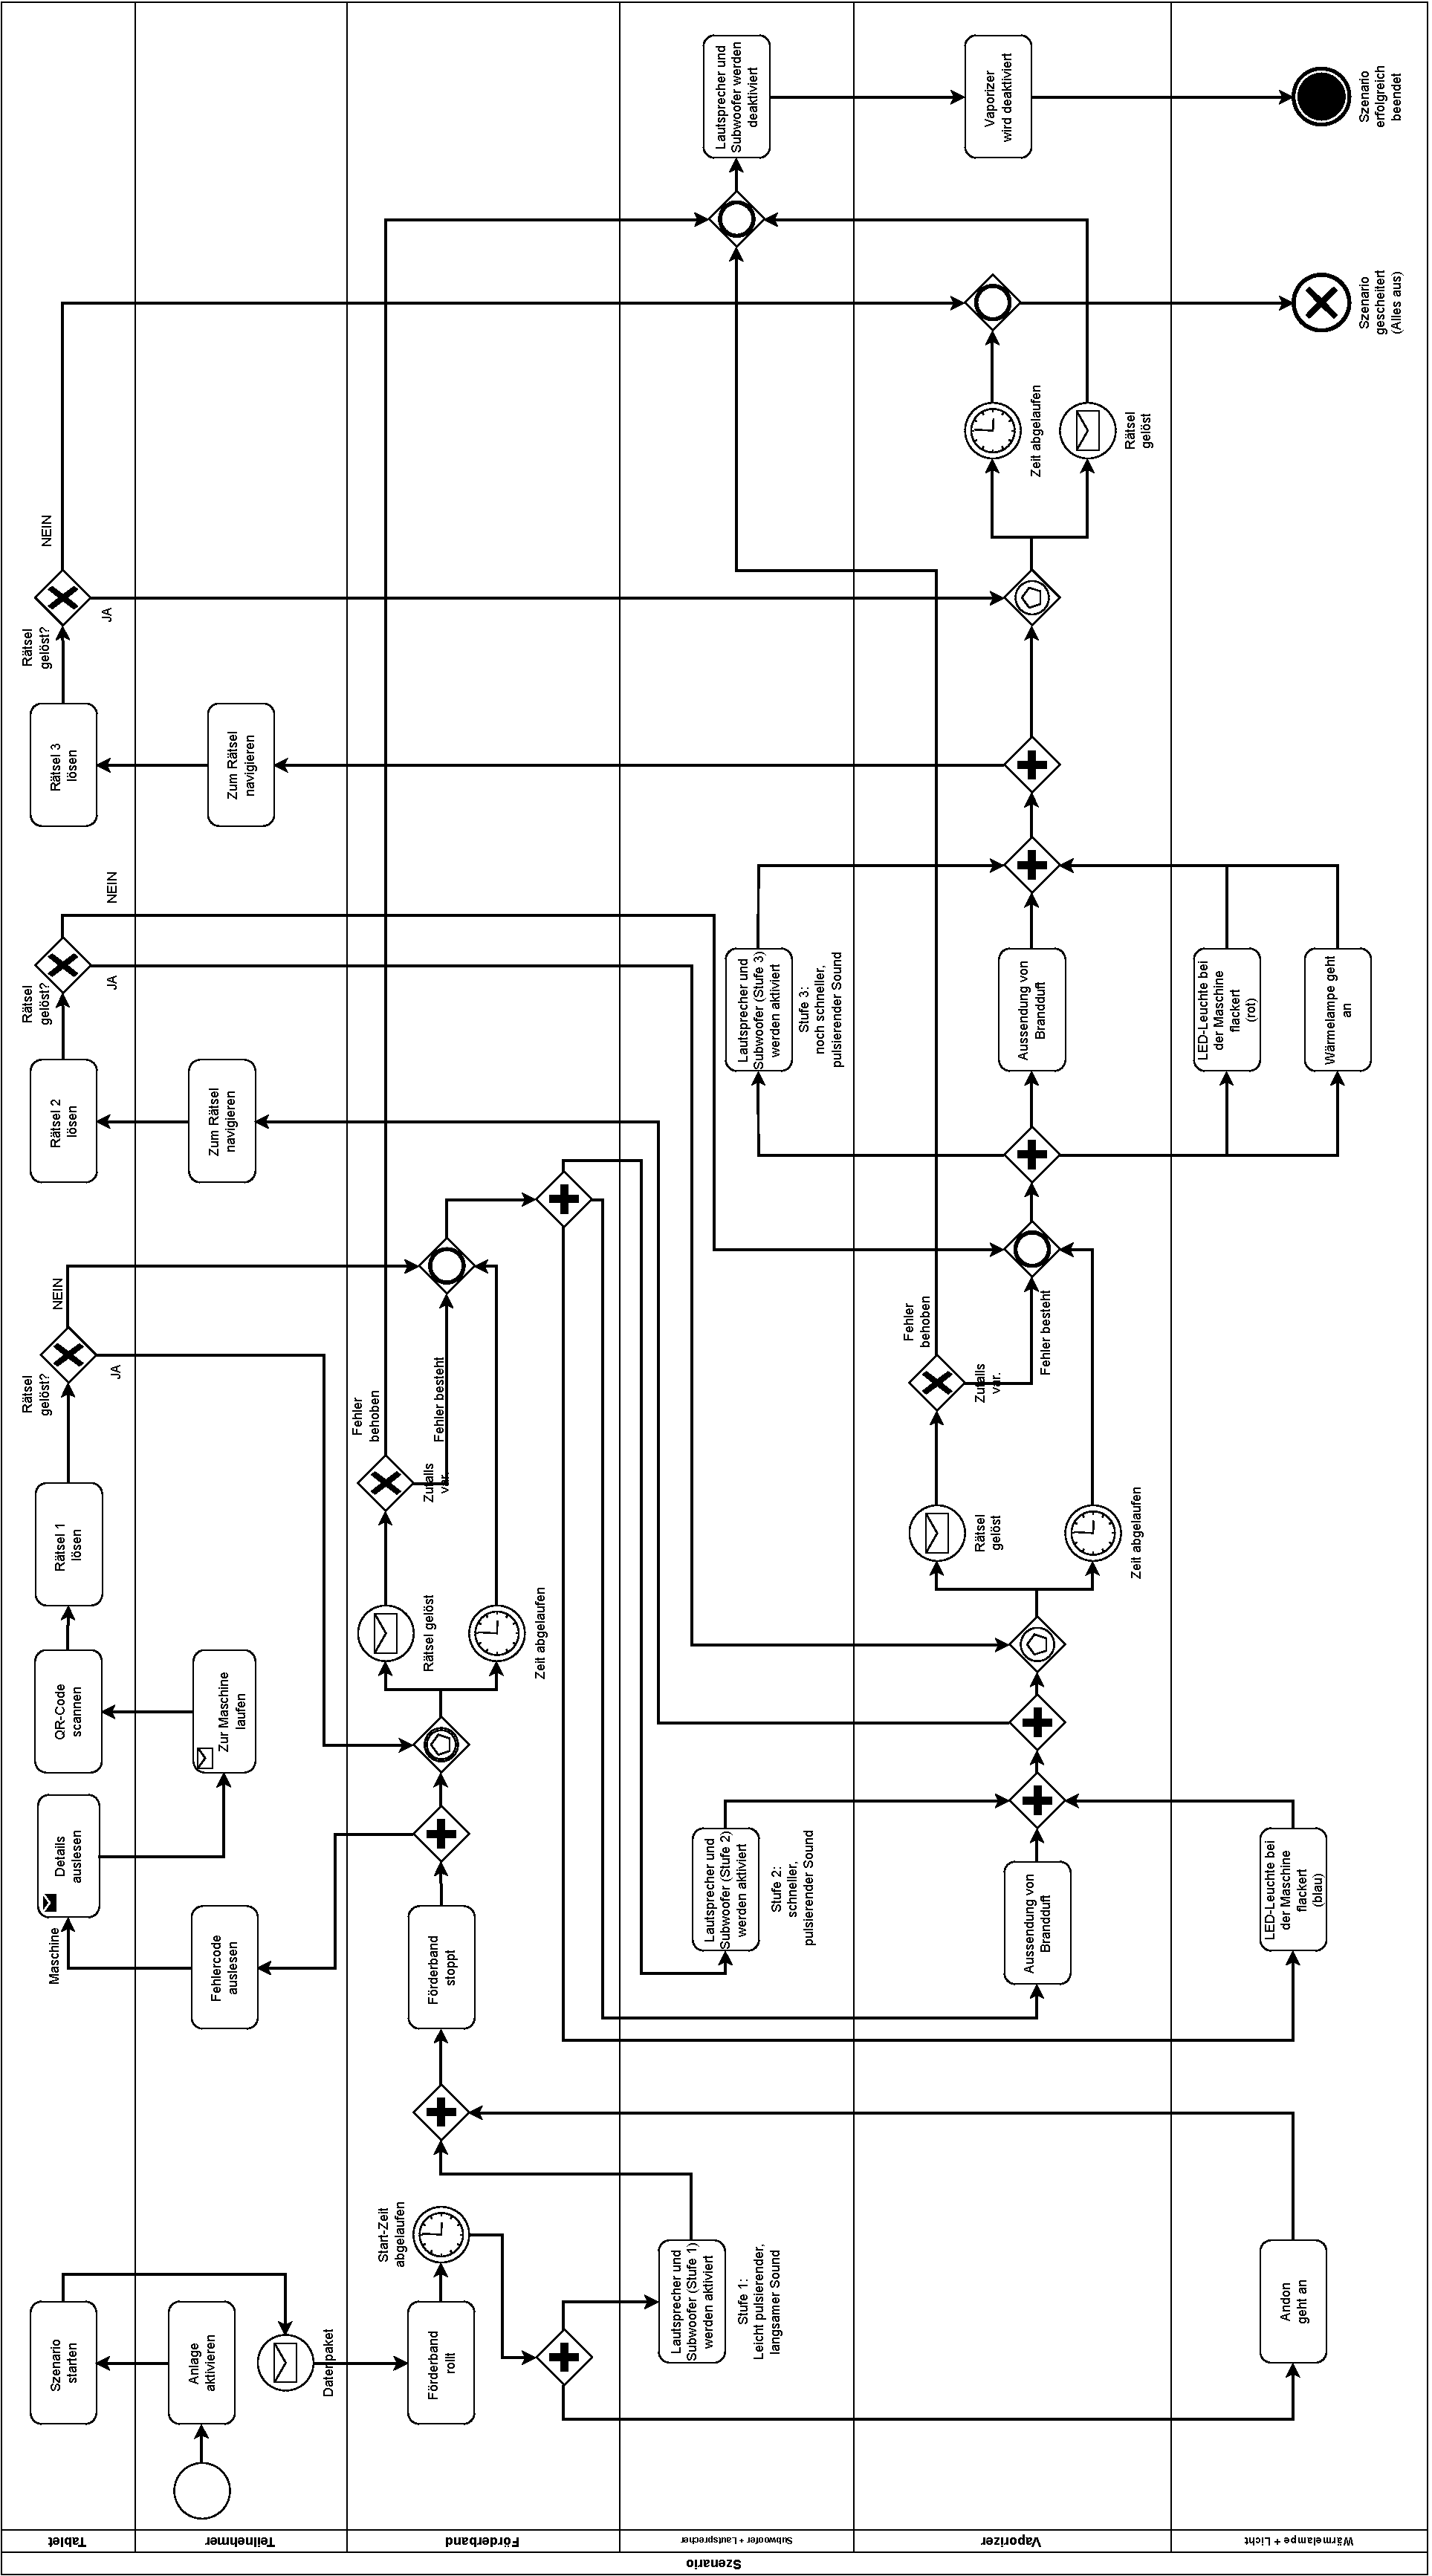
\includegraphics[scale=0.37]{res/Finales Szenario BPMN(korrigiert).drawio-5.pdf}
    \caption{BPMN-Diagramm}
\end{figure}

Die nachfolgende Abbildung veranschaulicht den detaillierten Ablauf des Szenarios in Form eines BPMN-Diagramms mit insgesamt sechs Swimlanes. Dabei repräsentieren die Swimlanes die Komponenten ''Tablet'', ''Teilnehmer'' und ''Förderband''.

Die Komponenten, die im Verlauf des Szenarios zur Immersion genutzt werden, sind entsprechend ihrer Wahrnehmungsart in drei unterschiedliche Swimlanes aufgeteilt. Die Swimlane \textit{Subwoofer+Lautsprecher} widmet sich den auditiven Komponenten, während die Swimlane \textit{Vaporizer} die Geruchs-Aspekte des Szenarios skizzieren. Zusätzlich bezieht sich die Swimlane \textit{Wärmelampe+Licht} auf die Prozesselemente mit visuellen Komponenten.


\begin{comment}
\section{Prozessmodellierung}

%Sätze beginnen alle mit Die...Die...Die. Evtl. abändern wenn euch eine bessere Formulierung einfällt.
Die folgende Abbildung stellt den detaillierten Prozessablauf des Szenarios in Form eines BPMN-Diagramms dar. \\
Das Diagramm besteht aus sechs Swimlanes. Die Komponenten „Tablet“, „Teilnehmer“ und „Förderband“ werden durch je eine Swimlane abgebildet. Die im Laufe des Szenarios zur Immersion eingesetzten Komponenten sind nach der Art ihrer Wahrnehmung in drei verschiedene Swimlanes unterteilt. Die Swimlane „Subwoofer+Lautsprecher“ bezieht sich auf den die auditiven Komponenten. Die Swimlane „Vaporizer“ beschreibt die Elemente des Szenarios mit Bezug auf olfaktorische Wahrnehmung. Die Swimlane „Wärmelampe+Licht“ bezieht sich auf die Prozesselemente mit visuellen Komponenten.


\begin{figure}
    \caption{BPMN-Diagramm}
    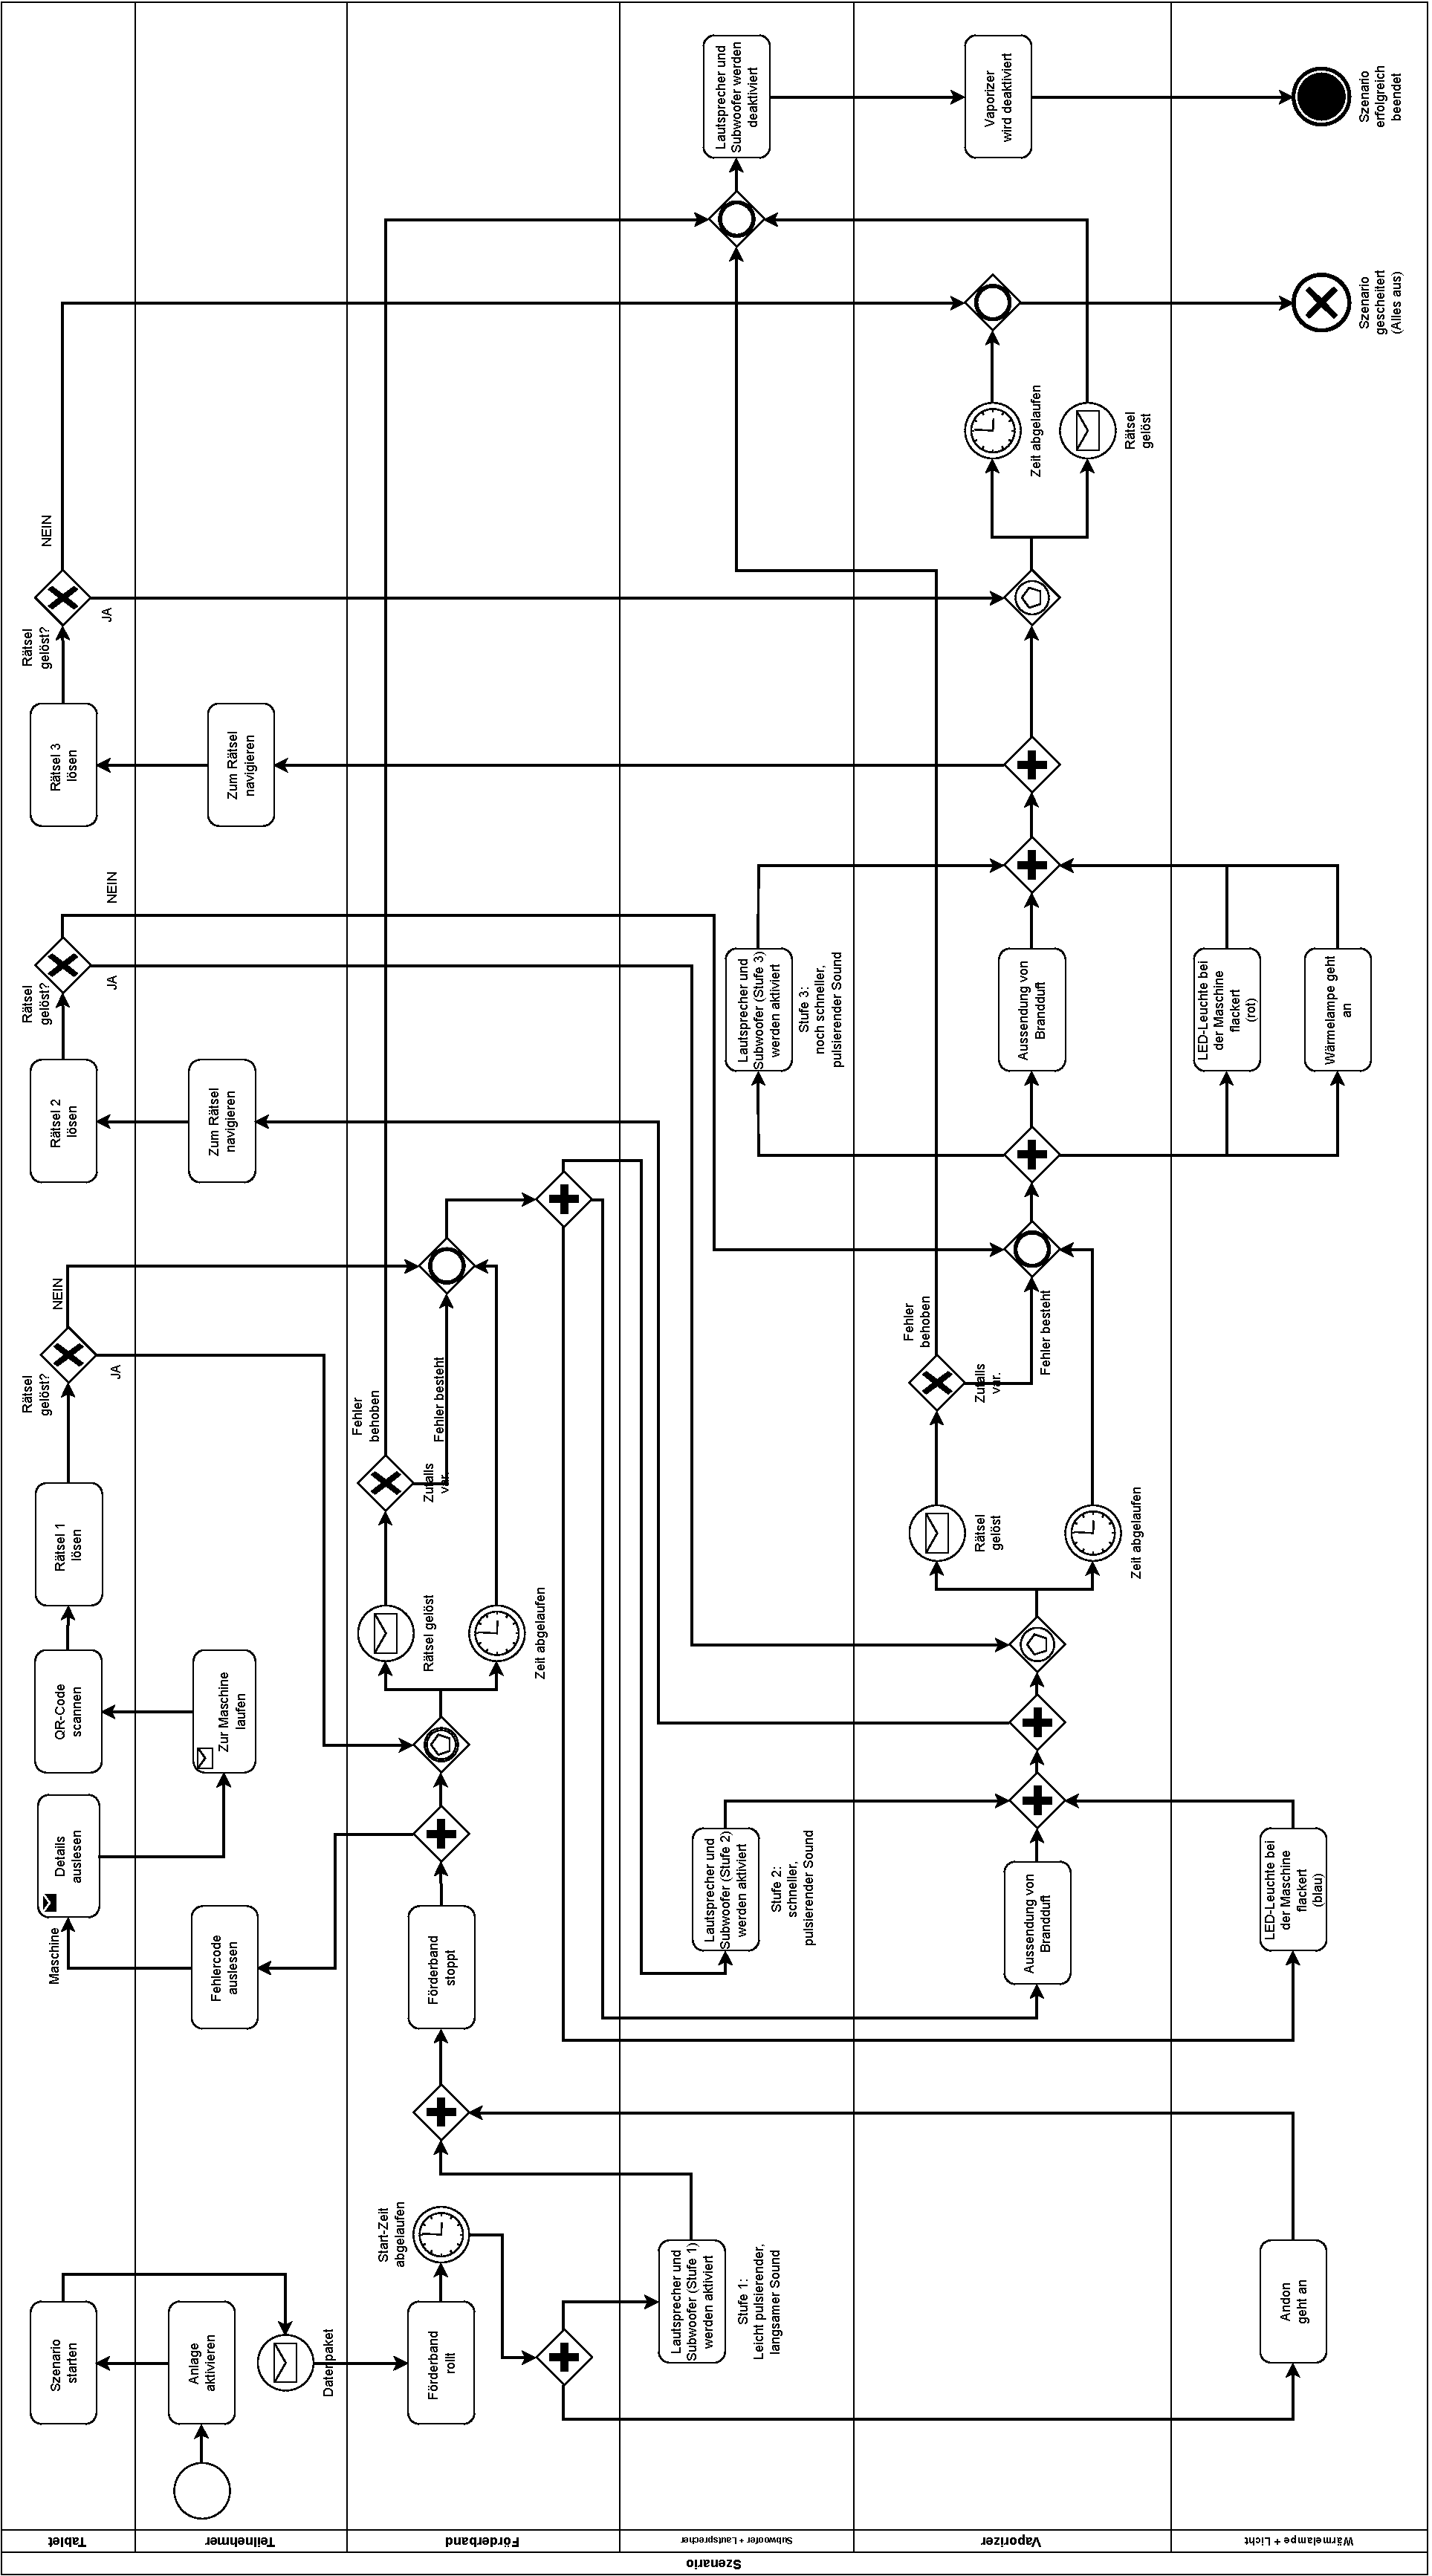
\includegraphics[scale=0.37]{res/Finales Szenario BPMN(korrigiert).drawio-5.pdf}
\end{figure}
\end{comment}